\documentclass[11pt,a4]{jsarticle}

\input{include/macro.tex}
\input{include/preamble.tex}

\begin{document}
  \begin{titlepage}

  \vspace*{25mm}

  \begin{center}
    {\huge 知能制御PBL\\}
    \vspace{5mm}
    {\Huge 第2回RCR中間報告\\}
    \vspace{20mm}
    {\Large 2017年5月31日}

    \vspace{25mm}

    {\LARGE 西田研究室\\}

    \vspace{10mm}

    {\Large
   13104042 烏谷崇大  \\
   14104043 桑野僚大  \\
   14104034 下松八重宏太\\
   14104090 中尾真人  \\
   14104111 本田空   \\
   14104131 山崎達也  \\
   16104313 山下翔   \\
}

  \end{center}

\end{titlepage}


\newpage
  \tableofcontents

\newpage
\section{目的} \setcounters{0}

  学部3年までに学習した制御理論や電気回路・情報工学の知識を使って,競技場内を自律的に走行するロボットの製作を行う.
  研究室で一丸となってプロジェクトを進行し,共同で課題を達成することの難しさや楽しさを学び,
  エンジニアとして仕事を進めるための素養を身に付ける.

\section{競技概要} \setcounters{0}

  \subsection{ルール}
    競技場には障害物に見立てた黄色のポールや火災に見立てた赤色のポールが複数設置されている.
    ポールに接触せず,可能な限り速やかに火災を鎮火させる消防ロボット(ロボカー)を作成する.

  \subsection{競技場}
    競技場の全体図を\refig{picture/course.eps}に示し,以下に詳細を説明する.

    \begin{enumerate}
      \item 競技場は板張りの床であり,縦・横ともに$5400\unit{mm}$である.
      \item 競技場には黄色の固定ポールと赤色の火災ポールが設置されており,スタートからゴールまで,
            固定ポールには接触,火災ポールには衝突することなく通過しなければならない.
      \item 火災ポールは青色の鎮火ポールに赤色の幕を被せたものであり,上部におもりなどを落としたり,
            幕を剥がしたりすることで鎮火ポールに変化させる(このポールの製作も行うこと).
      \item スタート後は右手に固定ポールを見ながら直進し,消火活動開始区間まで移動しなければならない.
            消火活動開始区間に進入後は,右折し火災ポールを発見し次第消火にあたる.
      \item すべての火災ポールを消火し,鎮火ポールに変化させた後,ゴール地点で停止する.
      \item 火災ポールの配置は競技ごとに異なる.また,鎮火ポールが存在することもある.
      \item ポールは直径$80\unit{mm}$・高さ$120\unit{mm}$の中空パイプであり,黄・赤・青の色が付けられている.
    \end{enumerate}

    \labeledfigure{H}{0.9}{picture/course.eps}{2017年度 RCR走行コース}

\section{機体概要} \setcounters{0}

  我々は本機を,競技達成を目的としつつも,
  機体・プログラムともに来年度以降のRCRにも最小限の修正で再利用できることも期待して,
  競技ルールに対して特化した機体構造としないことを念頭に置いて設計した.

  そのため,ポールを数えるなどの処理を実装せず,自己位置推定により得られた競技場内の座標から,事前に設定した擬似的な地図情報を利用して進行方向を決定する.
  また,全周に配置した測距センサにより周囲のあらゆる物体から適切な距離を保つように機体を振る舞わせる物体回避が常に働いており,進行方向に自然な修正舵があてられる.

  炎上ポールへの接近は画像処理を元に算出したベクトルが進行方向を置き換える形で設定され,物体回避と接近が釣り合うことで炎上ポールの寸前で停止する.
  消火活動は炎上ポールを前に停止することを条件に開始され,消火活動により目の前から炎上ポールが消えることで,探索行動へ復帰する.

\section{走行アルゴリズム} \setcounters{0}

  機体の進行方向及び速度は人工ポテンシャル法により制御を行う.

  目標方向として,赤い物体へ向かうベクトル$\bm{v}_{\rm{red}}$または順路に沿ってゴールへ向かうベクトル$\bm{v}_{\rm{goal}}$を与える.
  また,障害物回避のためポテンシャル場を設定する.\\

  二次元平面上の円筒状の障害物(ポール)$p_i$について,機体の回転中心を原点にスカラー場$f_i$を設定する.

  \begin{equation}
    f_i(x,y) = - \tanh^{-1}(x^2 + y^2 - 1)
  \end{equation}

  次に障害物$p_i$のスカラー場の勾配として表されるベクトル場は次のようになる.
  ただし,$\hat{x}$,$\hat{y}$はそれぞれ$x$,$y$軸方向の単位ベクトルである.

  \begin{equation}
    \frac{\partial f_i}{\partial x}\hat{x} + \frac{\partial f_i}{\partial y}\hat{y} = \nabla f_i(x,y)
  \end{equation}

  しかし,実際の機体はコース上の全障害物の位置を常に把握しておくことは不可能であり,
  測距センサの検出距離にも限りがあることから,
  機体から半径$d_{\rm{max}} = 0.9 \unit{m}$の範囲内のポールについてのみベクトル場を考慮している.

  測距センサにより得られたポール$p_i$へのベクトルを$\bm{d}_i = [d_{ix}, d_{iy}]^{T}$とすると,
  機体がポールから受ける斥力$\bm{F}_i$は次のように表せる

  \begin{equation}
    \bm{F}_i = \nabla f_i(\frac{d_{ix}}{d_{\rm{max}}}, \frac{d_{iy}}{d_{\rm{max}}})
  \end{equation}

  以上より,範囲内に$n$個ポールが存在する場合の機体の進行方向$\bm{v}$は次のように表せる.

  \begin{equation}
    \bm{v} = \frac{\bm{v}_{\rm{target}}}{\|\bm{v}_{\rm{target}}\|} + \frac{\sum_{i=0}^{n-1}{\bm{F}_i}}{\|\sum_{i=0}^{n-1}{\bm{F}_i}\|}
  \end{equation}

  $\bm{v}_{\rm{target}}$には,$\bm{v}_{\rm{red}}$と$\bm{v}_{\rm{goal}}$のどちらかが設定される.
  機体正面のカメラにより撮影された画像を元に$\bm{v}_{\rm{red}}$が生成されている場合はそれが,
  ない場合は$\bm{v}_{\rm{goal}}$が設定される.\\

  $\bm{v}_{\rm{red}}$は撮影した画像から赤色物体を抽出し,機体中心から赤色物体の画像重心へ向かうベクトルをカメラの画角を元に算出する.
  $\bm{v}_{\rm{goal}}$は概念上はスタート地点からゴール地点への下り坂となるようなスカラー場から勾配ベクトルを取り出すことによって得られるとしているが,
  実際は処理の簡単のため,競技場を$0.9\unit{m}$毎に区切ったグリッドに対して定義したベクトル場から直接ベクトルを得ている.\\

  なお,$\bm{v}_{\rm{target}}$に$\bm{v}_{\rm{red}}$が設定された場合,機体は赤い物体の直前で$\bm{v} = [0, 0]^{T}$となり停止する.
  これを消火作業を行うための条件とし,消火作業により機体正面のカメラから赤色の物体が消えることで消火作業が終了する.

\section{機械設計} \setcounters{0} % TODO

  % 西田研究室では今回製作するロボカーの構成要素のうち,
  % 制御手法,構成パーツ(センサなど),機体設計の順に重要度の順位を定めた.
  % そのため各パートの担当者と打ち合わせをしながら機体の設計を行った.
  機体設計にはAutodesk社のCADソフトAutodesk Inventor Professional 2018(以下,Inventor)を使用した.

  \subsection{1号機}
    最初にInventorで設計した1号機を\refig{picture/first_assembly.eps}に示す.
    機体のサイズは幅$300\unit{mm}$,高さ$120\unit{mm}$とした.
    センサを均等に配置するために機体の形を正八角柱にし,
    1階部分を駆動系,2階部分をセンサ系,3階部分をアームやマイコン,カメラを置く空間とした.

    % この頃の設計はロボカーの制御手法や構成パーツについてあいまいな点が多く残っていたため,
    % 急な変更に対応できるようスペースを多くとるように心掛けた.
    細かな仕様変更を想定して空間に余裕を持たせていため,1号機は2号機に比べて各寸法が大きくなっている.

    \labeledfigure{H}{0.7}{picture/first_assembly.eps}{1号機の概観}

  \subsection{2号機}
    % 制御手法や構成パーツについての考えが固まってきた段階で,1号機の設計を元に再設計を行った.
    2号機の概観を\refig{picture/second_assembly.eps}に示す.
    % 再設計を行う際に各パートからの機体の要求条件を再度リストアップしてから行った.

    \subsubsection{設計要求}
      ソフト班から求められる機体の構成
      \begin{itemize}
       \item 制御のしやすい駆動系
       \item 回転半径の縮小
       \item センサの測定領域の均一化
       \item センサの取り付け位置(床面からの高さ)
      \end{itemize}

      回路班から求められる機体の構成
      \begin{itemize}
       \item 整備のしやすい設計
       \item 配線への考慮
      \end{itemize}

      \labeledfigure{H}{0.7}{picture/second_assembly.eps}{2号機の概観}

    \subsubsection{モータとエンコーダの配置}
      一号機の駆動系を\refig{picture/kuwano3.eps}に示す.
      一号機ではモータとエンコーダの配置を線対称としていたため,機体の幅が大きくしなければならなかった.
      そこで二号機ではこのモータとエンコーダの配置を点対象とすることにした.
      これによりタイヤのトレッド幅を限りなく小さくでき,機体の幅を小さくすることができた.
      また,一号機ではモータとエンコーダをアルミ板で下から支えるようになっていた.
      そのため,モータとエンコーダを支える以外のスペースは無駄なスペースとなっていた.
      二号機ではこの無駄なスペースを省くために,モータとエンコーダを上から支えることにした.
      上から支えるにしたがって,
      モータとエンコーダの重量と機体の荷重が\refig{picture/kuwano4.eps}に示した部分に集中する恐れがあるため,
      機体中心部分にモータおよびエンコーダを支えるパーツを3Dプリンタで作成し設置した.
      以上により,下から支えていたアルミ板を廃止することができ,一号機での無駄なスペースを削減することができた.

    \subsubsection{回路のガードについて}
      機体の大部分はアルミでできているため,回路を露出させたまま配置するとショートする危険性がある.
      したがって,回路をホットボンドで覆った.
      Arduinoに関しては専用のケースが存在しないため,3Dプリンタでケースを作成した.

    \subsubsection{タイヤについて}
      一号機では\refig{picture/kuwano5.eps}のようなタイヤを使用していたが,
      このタイヤは中身がスポンジになっており,機体の重量でタイヤの接地面積が増えやすく,
      また機体の荷重移動によって機体がロールする可能性があると考えた.
      二号機ではそういった問題を解消するべく,ナロータイヤを使用することにした.
      使用するナロータイヤを図\refig{picture/kuwano6.eps}に示す.
      使用するナロータイヤは非常に細いため,地面との接地面積を少なくすることができる.
      また,ゴムのみでできているので,一号機で使用する予定であったタイヤに比べて沈む量が少なく,
      機体の荷重移動によるロールも低減できると考えられる.
      しかし,接地面が小さくなったことでスリップする可能性があると考えられるので,
      キャンバー角をつけるなどして対策を考えていく.

    \labeledfigure{H}{0.6}{picture/kuwano3.eps}{1号機の駆動系}
    \labeledfigure{H}{0.6}{picture/kuwano4.eps}{最も荷重がかかる位置}
    \labeledfigure{H}{0.6}{picture/kuwano5.eps}{1号機のタイヤ}
    \labeledfigure{H}{0.6}{picture/kuwano6.eps}{2号機のタイヤ}

  \subsection{炎上ポール}
    当初,我々が設計したした消火ポールは,
    塩化ビニル管に青い布を巻きつけて鎮火ポール,その上から赤い布を覆うことで炎上ポールとし,
    ロボットアームによりポールの上から赤い布を塩ビ管の中に押し込むことで赤色の部分をカメラから不可視にするというものであったが,
    実際に作成してみて以下の欠点が挙げられた.
    \begin{description}
      \item 赤い布で青ポールを綺麗に隠せない
      \item 布を押し込む力が弱いとポールの中に入らない
      \item 布の中心を押し込む必要がある
      \item 布が長すぎてポールの中に入っても外に飛び出してしまう
    \end{description}
    そこで設計を変更し,鎮火ポールの周りに短冊状の裏表がそれぞれ赤と青の紙片を貼り付け,紙が自重によって裏返ることで消火とするよう修正した.
    完成した炎上ポールを\refig{picture/poll.eps}に示す.
    また,紙片の固定には弱い磁石をしようしている.

    \labeledfigure{t}{0.8}{picture/poll.eps}{完成した消火ポール}

  \subsection{消火機構} \setcounters{0} % TODO
    % アームは垂直方向に上下する1リンク機構を考える.
    % これは,消火方法がストッパを外すという単純なものであるからだ.

    アームの動作には,往復スライダ・クランク機構を採用する(\refig{picture/slide_clank.eps}).
    これは,回転運動を直線運動に変換する機構であり,
    回転はローテーションモータGWS S35 STDから得る.
    クランク腕長さを$r$,連接棒長さを$l$とするとその理想的なリンク比$\rho$は,
    \begin{equation}
      \rho = \frac{r}{l}=\frac{1}{3}
    \end{equation}
    とされている.

    今回は必要なストローク長が$80\unit{mm}$であったので,それぞれ$r=20\unit{mm}$,$l=60\unit{mm}$とした.
    実際に製作したアームを\refig{picture/arm_left.eps},\refig{picture/arm_right.eps}に示す.

    \labeledfigure{H}{0.4}{picture/slide_clank.eps}{消火用アーム概念図}

    \begin{tabular}{c}
      \begin{minipage}{0.45\hsize}
        \labeledfigure{H}{1.0}{picture/arm_left.eps}{アーム左面}
      \end{minipage}
      \begin{minipage}{0.45\hsize}
        \labeledfigure{H}{1.0}{picture/arm_right.eps}{アーム左面}
      \end{minipage}
    \end{tabular}

    % \subsection{使用モータ}
    %   ローテーションモータ(\refig{picture/servo.eps})の仕様について示す.
    %
    %   [GWS S35 STD]
    %   \begin{itemize}
    %    \item トルク        : 4.1 [kg] (@4.8 [V])
    %    \item スピード      : 0.27 [sec]/60[deg] (@4.8 [V])
    %    \item 重量          : 41 [g]
    %    \item サイズ        :$39.5 \times 20 \times 35.6$[mm]
    %   \end{itemize}
    %
    %   \labeledfigure{H}{0.5}{picture/servo.eps}{ローテーションモータ GWS S35 SSTD}

\section{回路設計} \setcounters{0} % TODO

  設計・作成した回路について仕様や選定理由について以下に示す.
  また使用する部品の一覧を\reftab{circuit_parts}に示す.

  \subsection{マイコンの選定}
    設計した回路を\refig{picture/circuit_raspi.eps},\refig{picture/circuit_arduino.eps}に示す.
    マイコンとしてRaspberry Pi 3 Model B(以下 Raspberry Pi)とArduino Uno R3(以下 Arduino)を使用する.
    Raspberry Piは複雑な処理を行う上で,オペレーティングシステムの支援を受けることが出来る点,
    また,処理速度についてCPU$1.2\unit{GHz}$,RAM$1\unit{GB}$とArduinoの$16\unit{MHz}$,$32\unit{KB}$と比べて大きく優れている点から,並列処理や画像処理に適しているため採用した.

    Raspberry PiはアナログI/Oポートを装備しておらず,アナログ出力のセンサ処理が困難であるため,アナログ ディジタルI/Oポートを持つArduinoにカメラ以外のセンサ処理を一括して行わせる.
    ただし,必要なアナログI/Oポート数が後述の$\mathrm{I^2C}$通信を使用しても足りないため,Arduino用16チャンネル アナログ マルチプレクサによりアナログI/Oポートの増設を行った.

    \begin{table}[h]
      \centering
      \caption{回路用部品表}
      \begin{tabular}{|l|c||l|} \hline
        部品名                 & 数量 & 備考                                               \\ \hline \hline
        Raspberry Pi 3 model B & 1    & 高次の計算・画像処理・モータ制御                   \\ \hline
        Arduino Uno R3         & 1    & センサの読み取り,自己位置推定                     \\ \hline
        AO-8014                & 2    & DCギアードモータ                                   \\ \hline
        GWS S35 STD            & 1    & ローテーションモータ                               \\ \hline
        MD10C-R3               & 2    & モータドライバ                                     \\ \hline
        CD74HC4067             & 1    & ArduinoアナログI/Oピン増設用アナログマルチプレクサ \\ \hline
        PCA9306                & 1    & $\mathrm{I^2C}$通信用変換モジュール                \\ \hline
        GP2Y0A02YK             & 7    & PSD測距センサ                                      \\ \hline
        VL6180x                & 3    & ToF測距センサ                                      \\ \hline
        P5V04A                 & 1    & Raspberry Piカメラモジュール                       \\ \hline
        KXR94-2050             & 1    & 3軸加速度センサ                                    \\ \hline
        BGD20                  & 1    & 3軸ジャイロセンサ                                  \\ \hline
        LT8697                 & 1    & $7.2\unit{V}$ $\rightarrow$ $5.0\unit{V}$ $2500\unit{mA}$降圧レギュレータ \\ \hline
        BTD05-05S200D          & 1    & $7.2\unit{V}$ $\rightarrow$ $5.0\unit{V}$ $2500\unit{mA}$降圧レギュレータ \\ \hline
        電解コンデンサ $47\unit{\mu F}$ & 2 & 電源安定化                                   \\ \hline
        セラミックコンデンサ $0.1\unit{\mu F}$ & 9 & 信号安定化(ローパスフィルタ回路)    \\ \hline
        POWER MAX 4000 Ni-MH   & 1    & 電源バッテリー $7.2\unit{V}$ $4200\unit{mAh}$      \\ \hline
      \end{tabular}
      \label{label::table::circuit_parts}
    \end{table}

    \labeledfigure{H}{0.9}{picture/circuit_raspi.eps}{Raspberry Pi 3 接続回路図}
    \labeledfigure{H}{0.9}{picture/circuit_arduino.eps}{Arduino uno R3 接続回路図}

  \subsection{モータドライバ}
    モータドライバはMD10C R3(\refig{picture/md10c.eps})を両輪駆動用として2つ使用する.
    その仕様を次に示す.

    \begin{description}
      \setlength{\leftskip}{3mm}
      \item[MD10C RC] \mbox{} \\
        電源電圧:$\mathrm{DC}5\unit{V} \sim 25\unit{V}$ \\
        最大電流:$13\unit{A}$ \\
        ロジック電源:モータ用電源より供給 \\
        ロジック電圧:$\mathrm{DC}5\unit{V} または 3.3\unit{V}$
    \end{description}

    \labeledfigure{H}{0.6}{picture/md10c.eps}{MD10C R3}

  \subsection{センサ仕様}
    ロボットに搭載されているセンサを以下に列記する.
    \begin{description}
      \setlength{\leftskip}{3mm}
      \item[赤外線測距センサ(GP2Y0A025YK)] \mbox{} \\
        有効距離$20 \sim 150\unit{cm}$
      \item[ToF近距離センサ(VL6180x)] \mbox{} \\
        有効距離$5 \sim 20\unit{cm}$
      \item[3軸加速度センサ(KXR94-2050)] \mbox{} \\
        3軸加速度出力
      \item[ジャイロセンサ(BGD20)] \mbox{} \\
        3軸角加速度出力
      \item[カメラモジュール(P5V04A)] \mbox{} \\
        Raspberry Pi用カメラ
    \end{description}

    \subsubsection{測距センサ}
      測距センサは本体周囲にPSDセンサを7つ,前方にToF近接センサを3つ搭載する(\refig{picture/distance_sensors.eps}).
      これは自律行動の際に周辺環境,特に各種ポールを把握するために用いる.
      このとき,近接センサは$\mathrm{I^2C}$通信によって使用する.

      また,各測距センサには信号のノイズを吸収し安定化させるために$0.1 \unit{\mu F}$のセラミックコンデンサを接続する.
      これは,コンデンサの持つ交流成分のみを吸収し,直流成分を通すというローパスフィルタ的特徴を利用したものである.

      \labeledfigure{b}{0.5}{picture/distance_sensors.eps}{上:PSDセンサ 下:ToFセンサ}

    \subsubsection{3軸加速度・ジャイロセンサモジュール}
      加速度センサは3軸におけるロボットの加速度を測定するものである.
      ジャイロセンサは3軸まわりの角加速度を測定するものである(\refig{picture/gyro_sensor.eps}).

      我々はこれらをロボットの自己位置推定に用いる.
      特にジャイロセンサについては,ロボット本体の直進走行制御に使用する.

      \labeledfigure{t}{0.4}{picture/gyro_sensor.eps}{3軸加速度・ジャイロセンサモジュール}

  \subsection{電源回路}
    電源回路は各回路図の左上に示している.
    バッテリーはひとつしか搭載しないが,Raspberry PiとArduinoでは定格電流値が異なるために同一の電源は使用できない.
    そこで,それぞれに降圧レギュレータとしてDCDCコンバータを用いてバッテリーからの供給電源を分電することとした.
    各仕様を以下に示す.
    また,実際に作成した電源回路を\refig{picture/power_supply.eps}に示す.

    \begin{description}
      \setlength{\leftskip}{3mm}
      \item[LR8697] \mbox{} \\
        電源電圧:$\mathrm{DC}6.0\unit{V} \sim 42.0\unit{V}$ \\
        出力電圧:$\mathrm{DC}5.0\unit{V}$ \\
        出力電流:$\mathrm{DC}2500\unit{mA}$ \\
    \end{description}

    \begin{description}
      \setlength{\leftskip}{3mm}
      \item[BTD05-05S200D] \mbox{} \\
        電源電圧:$\mathrm{DC}4.5\unit{V} \sim 9.0\unit{V}$ \\
        出力電圧:$\mathrm{DC}5.0\unit{V}$ \\
        出力電流:$\mathrm{DC}2000\unit{mA}$ \\
    \end{description}

    \labeledfigure{t}{0.4}{picture/power_supply.eps}{電源回路モジュール}

  \subsection{$\mathrm{I^2C}$通信}
    我々のロボットには測距センサを始めとする複数のセンサが搭載されている.
    これらの殆どがアナログ出力であるが,ArduinoはアナログI/Oポートは6つしか備えていないため要求を満たさない.

    そのため$\mathrm{I^2C}$通信を用いた.
    これは,$\mathrm{I^2C}$通信がパーティライン構成が可能となっており,
    1つのマスタで複数のスレーブデバイスと通信することが可能であるからである.
    概要を以下に示す.
    \begin{enumerate}
      \item マスタ側(Arduino)とスレーブ側(n個のセンサ等)を明確に分け,各スレーブに異なるアドレスを割り振る.
      \item マスタ側がStart Conditionを出力し続いてアドレスとRead/Write要求を出力する.
      \item 全スレーブがこの時のSCLのクロックを元にSDAのデータを受信し,SSPADDレジスタにセットされたアドレスと一致したデバイスだけが,その後の送受信を継続する.
      \item 受信した側がデータを受信完了すると自動的にACKビットを返送し,同時にSSP割込みを発生する.
      \item これをマスタがStop Conditionを出力するまで続ける.
    \end{enumerate}

    本機では近接センサ・ジャイロセンサについて$\mathrm{I^2C}$通信を行った.
    また,Arduinoと各デバイスはArduinoのSDA・SCLポートを使用することで通信が可能となる.
    これを実現するためにArduino用$\mathrm{I^2C}$バス用双方向電圧レベル変換モジュール
    (\ref{picture/level_transmittor.eps})を使用して接続した.
    接続の方法を回路図に示す.

    \labeledfigure{h}{0.4}{picture/level_transmittor.eps}{レベル変換モジュール}

  \subsection{回路作成}
    本機はセンサを計13個搭載している.
    そのため,それぞれの配線や配置は困難であった.
    電源管理では当初センサへの給電をArduinoから行っていたが,
    電流の不足からRaspberry Piとのシリアル通信が不安定になるという問題が生じた.
    そのため,電源回路からきちんと別電源を用意することとした.

    また,最大の問題となったのが配線である.
    全方位に搭載した各種センサのために機体内の配線が煩雑となってしまい,故障の原因となっていた.

    そこで,センサ配線のハブモジュールの作成や各種ピンのコネクタによる一元化を行うことで整理された配線となるように工夫した.

\section{センシング} \setcounters{0} % TODO

  \subsection{PSDセンサの選定} \setcounters{0} % TODO
    引き継ぎ物品の内2種類のPSDセンサから本機のセンサ用途により適した一方を選定する.
    選定に際しセンサ値-距離特性を求めるため同定実験を行った.

    実験対象の2種類のPSDセンサの仕様を以下に示す.
    また便宜上,仕様における最大測定距離から,それぞれを近距離センサ・遠距離センサと呼ぶ.

    \begin{description}
      \item[シャープ測距モジュール GP2Y0A21YK] \mbox{} \\
        範囲:$10 \sim 80\unit{cm}$ \\
        出力:アナログ電圧 \\
        寸法:$29.5 \times 13 \times 13.5\unit{mm}$ \\
        電源:$4.5 \sim 5.5\unit{V}$
    \end{description}

    \begin{description}
      \item[シャープ測距モジュール GP2Y0A02YK] \mbox{} \\
        範囲:$20 \sim 150\unit{cm}$ \\
        出力:アナログ電圧 \\
        寸法:$29.5 \times 13 \times 21.6\unit{mm}$ \\
        電源:$4.5 \sim 5.5\unit{V}$
    \end{description}

    \subsubsection{実験装置}
      PSDセンサの実験を行うため,\refig{picture/psded.eps}のような実験装置を製作した.
      PSDセンサは高さ$20\unit{mm}$の位置にセンサの発光部が左,受光部が右になるように箱に水平に装着した.
      PSDセンサの読み取りにはArduino Unoを用いた.
      % 実験時のセンサとArduinoの配線を図\refig{picture/psdwd.eps}に示す.
      実験時点ではポールが完成していなかったため,同等の径を持つ缶を用いた.

      \labeledfigure{t}{0.7}{picture/psded.eps}{PSD実験装置}
      % \labeledfigure{t}{0.7}{picture/psdwd.eps}{PSDセンサの配線図}

    \subsubsection{実験方法}
      PSDセンサの距離-出力電圧特性を測定するため以下の手順に従い実験を行った.
      \begin{enumerate}
        \item PSDセンサの発光部・受光部の先端を距離$0\unit{cm}$とし,
              近距離センサは$5\unit{cm}$から$100\unit{cm}$まで,
              $5\unit{cm}$ずつスプレー缶を移動させ出力電圧を記録する.
              このとき,スプレー缶の中心はPSDセンサの正面に置き測定する.
        \item 先程と同様に,遠距離センサは$5\unit{cm}$から$170\unit{cm}$まで,
              $5\unit{cm}$ずつスプレー缶を移動させ出力電圧を記録する.
      \end{enumerate}

    \subsubsection{実験結果}
      縦軸を出力電圧,横軸をPSDセンサ-対象物間の距離とし,
      近距離センサの測定結果のグラフを\refig{picture/psdn.eps}に,
      遠距離センサの測定結果のグラフを\refig{picture/psdf.eps}に示す.
      \refig{picture/psdn.eps}より,近距離センサは出力電圧が$40\unit{cm}$までは
      滑らかに減少しており,$40\unit{cm}$からは大きな変化は見られない.
      対して図\refig{picture/psdf.eps}より,遠距離センサは測距可能範囲内において
      出力電圧が$80\unit{cm}$までは滑らかに減少しており,
      $80\unit{cm}$からは変化に乏しいことがわかる.
      よって,近距離センサでは$40\unit{cm}$以降,遠距離センサでは$80\unit{cm}$以降の
      距離を算出することが難しくなると考えられる.
      ここで,今回のロボットは$40\unit{cm}$以降も距離を計測する必要がある.
      従って適当なセンサは,遠距離センサであると考えられる.

      \labeledfigure{H}{0.8}{picture/psdn.eps}{近距離センサ}
      \labeledfigure{H}{0.8}{picture/psdf.eps}{遠距離センサ}

  \subsection{センサのモデル化}
    プログラム上でセンサから読み取った値を扱えるようにするため,モデル化を行った.
    なお変数はそれぞれ,距離$d\unit{cm}$,加速度$a\unit{m/s^2}$,電圧$v\unit{V}$である.
    また,変数$i$はArduinoの\texttt{analogRead}関数により$0\sim1023$の値として正規化された$0\sim5\unit{V}$の電圧である.

    PSDセンサ(GP2Y0A21)について,モデル式を\refeq{GP2Y0A21}に示す.
    モデル化には\refig{picture/psdf.eps}のデータを用いた.
    \eq{GP2Y0A21}{ d = 45.514 i^{-0.822} }

    ToFセンサ(VL6180X)について,モデル式を\refeq{VL6180X}に示す.
    \eq{VL6180X}{ d = 0.09999 i + 0.4477 }

    加速度センサ(KXR-94)について,モデル式を\refeq{KXR-94}に示す.
    なお,電圧から減じている値はオフセット電圧である.
    \eq{KXR-94}{ a = 9.8 (v - 2.5) }

  \subsection{自己位置推定:車体角度}
    ジャイロセンサ(角速度センサ)を用いて,車体の角度を求める.角速度センサと同様に考える.
    角度を$\theta(t)\unit{deg}$,角速度を$\omega(t)\unit{deg/s}$とすると
    \eq*{ \theta(t) = \frac{t_2 - t_0}{6} (\omega(t_0) + 4 \omega(t_1) + \omega(t_2)) }
    となる.

  \subsection{自己位置推定:移動距離}
    加速度センサを用いて,移動距離を求める.
    そのために加速度センサから,加速度とそのときの時間を得る.
    今回は加速度を積分するために,数値積分のシンプソン公式を用いた.
    シンプソン公式による区間$(a,b)$の$f(t)$の積分値は以下のようになる.
    \eq*{ \int_a^b f(t) dt = \frac{b-a}{6} (f(a) + 4f (\frac{a+b}{2}) + f(b)) }
    これを用いて,$(t_0,t_2)$の区間で積分する(ただし$t_1=\frac{t_0+t_2}{2}$).

    $a(t)\unit{m/s^2}$を加速度,$v(t)\unit{m/s}$を速度とすると
    \eq*{ v(t) = \frac{t_2-t_0}{6} (a(t_0) + 4 a(t_1) + a(t_2)) }
    となる.よって移動距離を$x(t)\unit{m}$とすると以下のように表せる.
    \eq*{ x(t) = \frac{t_2-t_0}{6} (v(t_0) + 4 v(t_1) + v(t_2)) }

  \subsection{アフィン変換}
     加速度センサで得られる加速度はロボットのローカル座標系における加速度である.
     そこで,ジャイロセンサから得られた角度を用いて三次元アフィン変換を適用しグローバル座標系における加速度を求める.\\
     アフィン変換において,回転移動は次の行列で表される.
     $x$軸,$y$軸,$z$軸まわりの回転行列をそれぞれ$R_x, R_y, R_z$とおくと,

     \begin{eqnarray}
       R_x =
         \left[ \begin{array}{cccc}
           1 &        0       &       0       & 0 \\
           0 &  \cos \theta_x & \sin \theta_x & 0 \\
           0 & -\sin \theta_x & \cos \theta_x & 0 \\
           0 &        0       &       0       & 1
         \end{array} \right] \\
       R_y =
         \left[ \begin{array}{cccc}
           \cos \theta_y & 0 & -\sin \theta_y & 0 \\
                 0       & 1 &       0        & 0 \\
           \sin \theta_y & 0 &  \cos \theta_y & 0 \\
                 0       & 0 &       0        & 1
         \end{array} \right] \\
       R_z =
         \left[ \begin{array}{cccc}
           \cos \theta_z & \sin \theta_z & 0 & 0 \\
          -\sin \theta_z & \cos \theta_z & 0 & 0 \\
                 0       &       0       & 1 & 0 \\
                 0       &       0       & 0 & 1 \\
         \end{array} \right]
     \end{eqnarray}
     また,ローカル座標系の原点のグローバル座標系での座標を$(T_x, T_y, T_z)$とすると,
     アフィン変換における平行移動は次の行列で表される.
     \begin{equation}
      T =
        \left[ \begin{array}{cccc}
           1  &  0  &  0  & 0 \\
           0  &  1  &  0  & 0 \\
           0  &  0  &  1  & 0 \\
          T_x & T_y & T_z & 1 \\
        \end{array} \right]
     \end{equation}
     ここで,ローカル座標系を$(x, y, z, 1)$,グローバル座標系を$(x_g, y_g, z_g, 1)$とすると
     \eq*{ (x_g \  y_g \ z_g \ 1) = (x \ y \ z \ 1) R_z  R_x  R_y T }
     となる.これによってローカル座標系の加速度センサで得られた加速度をグローバル座標系に変換することが出来る.

  \subsection{フィルタ処理}
    \subsubsection{ローパスフィルタ}
      加速度センサやジャイロセンサで読み取った値は,ノイズが入り大きく上下していた.
      そこでセンサ値の平滑化を行うためローパスフィルタを用いた.
      ローパスフィルタの式を以下に示す.
      \eq{low_pass}{ y[i] = py[i-1] + (1-p)x[i] }
      ここで,$y[i]$は出力値,$y[i-1]$は前回の出力値,$x[i]$は現在のセンサ値であり,$p(0<p<1)$はパラメータである.
      この式の特徴として,パラメータ$p$を大きくすれば滑らかになるが,位相が遅れることがわかっている.

    \subsubsection{ハイパスフィルタ}
      センサ値をローパスフィルタで平滑化を行い,移動距離や回転角度を求めるためにその値の積分を行った.
      ここでの積分は数値積分であったため,積分誤差が生じ,時間とともに値がずれていた.
      これを解決するためにハイパスフィルタを用いた.ハイパスフィルタの式は以下に示す.
      \eq{high_pass}{ \acute{y}[i] = x[i] - y[i] }
      ここで,$\acute{y}[i]$は出力値,$x[i]$は現在の積分したセンサ値,
      $y[i]$は積分したセンサ値をローパスフィルタに通した出力値である.

  \subsection{画像処理}
    炎上ポールの認識には配布されたRapspberry Pi NoIR Camera V2(以下,カメラモジュール)を使用する.
    画像撮影から最も近いポールと思われる物体へのベクトルを出力する一連の手順を,簡単に以下に示す.
    画像処理にはOpenCVライブラリを用いており,各処理で使用した主要なライブラリ関数を併記する.

    \begin{description}

      \item[画像取得] \mbox{} \\
        カメラモジュールへのアクセスにはOpenCVとは異なる既成ライブラリ\cite{raspicam}を利用した.
        撮影により3チャンネルRGB画像データ(cv::Mat3b)が出力として得られる.
        実験により,競技会場で画像の撮影を行った場合炎上ポール以外の赤色の物体は画像の上半分にしか映らないことが判明しているため,
        取得した画像から下半分のみを切り出し,それに対して以下の処理を行う.\\

      \item[カラーモデル変換] \mbox{} \\
        得られた画像のカラーモデルをRGBからHSVに変換し,色相値のみを取り出す.
        赤色に対しての処理を簡単化するため,色相を180度回転させる.\\
        使用関数:\texttt{cv::cvtColor},\texttt{cv::split} \\

      \item[赤色強調] \mbox{} \\
        目標の色相値に対して赤の色相から遠いものほどより遠い色相に書き換えるフィルタを複数回反復して適用する.
        反復が終了した後,色相値0度を360度に書き換えるか,360度を0度に書き換える.\\
        使用関数:なし(おそらく既存の処理だが名前が分からないので自分で実装した) \\

      \item[ノイズ除去] \mbox{} \\
        モルフォロジー処理によりノイズを除去する.\\
        使用関数:\texttt{cv::morphologyEx} \\

      \item[構造解析] \mbox{} \\
        赤色が強調された画像からエッジを抽出した後,輪郭線を検出する.
        検出された輪郭線の内,面積最大のものを選択する.\\
        使用関数:\texttt{cv::Canny},\texttt{cv::findContours},\texttt{cv::contourArea} \\

      \item[ベクトル作成] \mbox{} \\
        選択した輪郭線の重心点を求め,カメラの画角($62.2 \times 48.8$ \cite{elinux})を元に機体中心から重心点へ向かうベクトルを作る.\\
        使用関数:\texttt{cv::moments} \\
    \end{description}

\section{競技結果と修正すべき点} \setcounters{0} % XXX 言い訳じみていてダサい

  競技会で我々の機体は課題を達成することが出来なかった.
  以下では,その原因について技術的な側面と開発体制の側面から考察を述べる.
  % もしそれが解消したとして次に直面することが予想される問題点について考える.

  \subsection{技術的な側面から考えられる原因}
    直接的な原因は自己位置推定が完成しなかったことである.

    本機のアルゴリズムはまず進行方向を必要とするが,
    それは事前に設定されたベクトル場から現座標のベクトルを取り出すことによって与えられる.
    赤い物体へ向かうベクトルを計算することは可能であったが,消火エリアへ機体を導く用途には使えないものである.
    つまり,自己位置推定により計算する予定であった競技場における機体の位置が分からない時点で,
    本機は動作アルゴリズムの根本から破綻した状態であった.

    そのため,競技会前日より進行方向を時間経過により変更させることで与えるようにアルゴリズムの変更を行ったが,
    目分量で計測した移動速度を元に設定した時間で管理しており,制御とは言えないものであった.
    また,仮に消火エリアに侵入できていたとしてもゴールへ帰還することは出来ない.
    さらにプログラム自体の設計を無視した急で歪な変更であったため,多くのバグを内包してしまっていた.

  \subsection{開発体制の側面から考えられる原因} % XXX 感想文的過ぎる
    ある程度ソフトウェア開発に慣れた人間同士であれば,インタフェースの仕様を定めておくだけで分担しての開発が行えるが,
    そうでない場合は作業分担は却って非効率であると考え,我々はプログラム開発を2人のみで行った.
    また,機械・電子回路の設計についても,それぞれに開発チーム内で突出して詳しい者が居たため設計・制作を一任した.

    最大の問題点は,それら開発の中核メンバーの全員が個人的な理由により,
    与えられた開発期間のおよそ半分もの間,開発に携われない状態になったことである.
    これは開発前より十分に予想が出来たことであるが,これ以外の開発体制を採用していた場合,
    今回の結果以上のものが出来たとは考えにくい.

    つまり,我々が競技会の課題を達成できなかった原因は,機体の設計目標を競技会の課題,
    そして開発チームの実力以上に高度に設定したことにあると考える.

    競技会の課題達成を目標とした場合は,本機のように複雑な処理を並列に繋げるよりも,
    何かを条件に進み・止まり・曲がるといった単純な処理を直列に繋げる設計の方が良い結果を出せたと考える.
    本機の最も複雑であった点はすべての処理が完璧に設計通りに動かなければ,まともに進むことすらままならないという点である.
    これが不具合箇所の特定と修正が困難となり,また,プログラムが肥大化した原因である.
    確実に動作する単純な処理を積み上げていったほうが,競技のクリアに段階的に近づけたはずである.

    より課題が複雑であった場合,例えば競技場が実際の街中であった場合などでは,恐らく我々の機体のような設計が優位となると考える.
    しかし,その場合はより分解能の高いセンサが必要となると考える.
    私は本機のアルゴリズムにおいて,
    レーザーレンジファインダやLiDARのような高度な測域センサを抽象化し極端に分解能を落としたものとして,
    測距センサを機体全周に配置したが,上手く働かなかった.
    上手く働かないのか,働かせることが出来なかったのかは勉強が足りないため分からない.

    私がこのRCRで学んだ最も大きなことは,
    課題にはその複雑さに応じた適当な複雑さのアルゴリズムが存在し,アルゴリズムは複雑さに応じたセンサの性能を要求するということである.
    我々は機体設計に置いてこのバランスを誤った.
    これが競技会の課題が達成できなかった根本的な原因であると考える.

  % \subsection{予想される問題点}
  %   以下では,本機のアルゴリズム・開発体制共に変更なく,無制限な開発期間が与えられていた場合,
  %   直面することが予想される問題点について述べる.
  %
  %   現時点で,そもそも本機はポールのような細い物体を認識できないという問題点がある.
  %   制御周期が長過ぎるために,ポールを測距センサが捉えられない,
  %   捉えられたとしても機体の進行方向へ一瞬しか影響を与えられない,とらえた時には既に衝突している,などである.
  %
  %   解決策は単純に制御周期を短くすることである.
  %   本機はプログラム実装において,実装の簡単や後の可読性・メンテナンス性を考慮して意図的に最適化を行っていない部分が多く存在する.
  %   典型的にはデータ管理にハッシュマップを多用していること,シリアル通信で数値データを送る際に一時的に文字列へ変換を行っていることが挙げられる.
  %   この節では無制限な開発期間を想定しているため,これらの最適化を十分に行えたとする.
  %
  %   それでも制御周期が長過ぎる場合,画像処理以外の計算処理をRaspberry Piから分離しH8などで行うことが必要である.
  %   設計時点ではこのような場合にはRaspberry Piから処理を分離すること無く,マルチスレッド処理により計算速度を確保することを計画していたが,
  %   後にそれが難しいことが判明している.
  %   具体的には,ARMプロセッサ向けの\texttt{libstdc++}のマルチスレッドライブラリのサポートが完全ではないことが問題である.
  %
  %   また,恒常的にCPUを$1\%$ほど使用するソフトウェアPWMを組み込みPWMに変更することも必要である.

\newpage
\section{物品一覧}

  本機に利用した引継ぎ品,配布品,購入品についてそれぞれ以降の表にまとめる.
  ただし,購入品について※印がついた部品は,購入はしたが使用しなかったものである.
  なお,合計金額は$\yen 76,786$である.

  \begin{table}[H]
    \centering
    \caption{引継ぎ品一覧}
    \includegraphics[width=1.0\hsize]{picture/items_inherited.eps}
  \end{table}

  \begin{table}[H]
    \centering
    \caption{配布品一覧}
    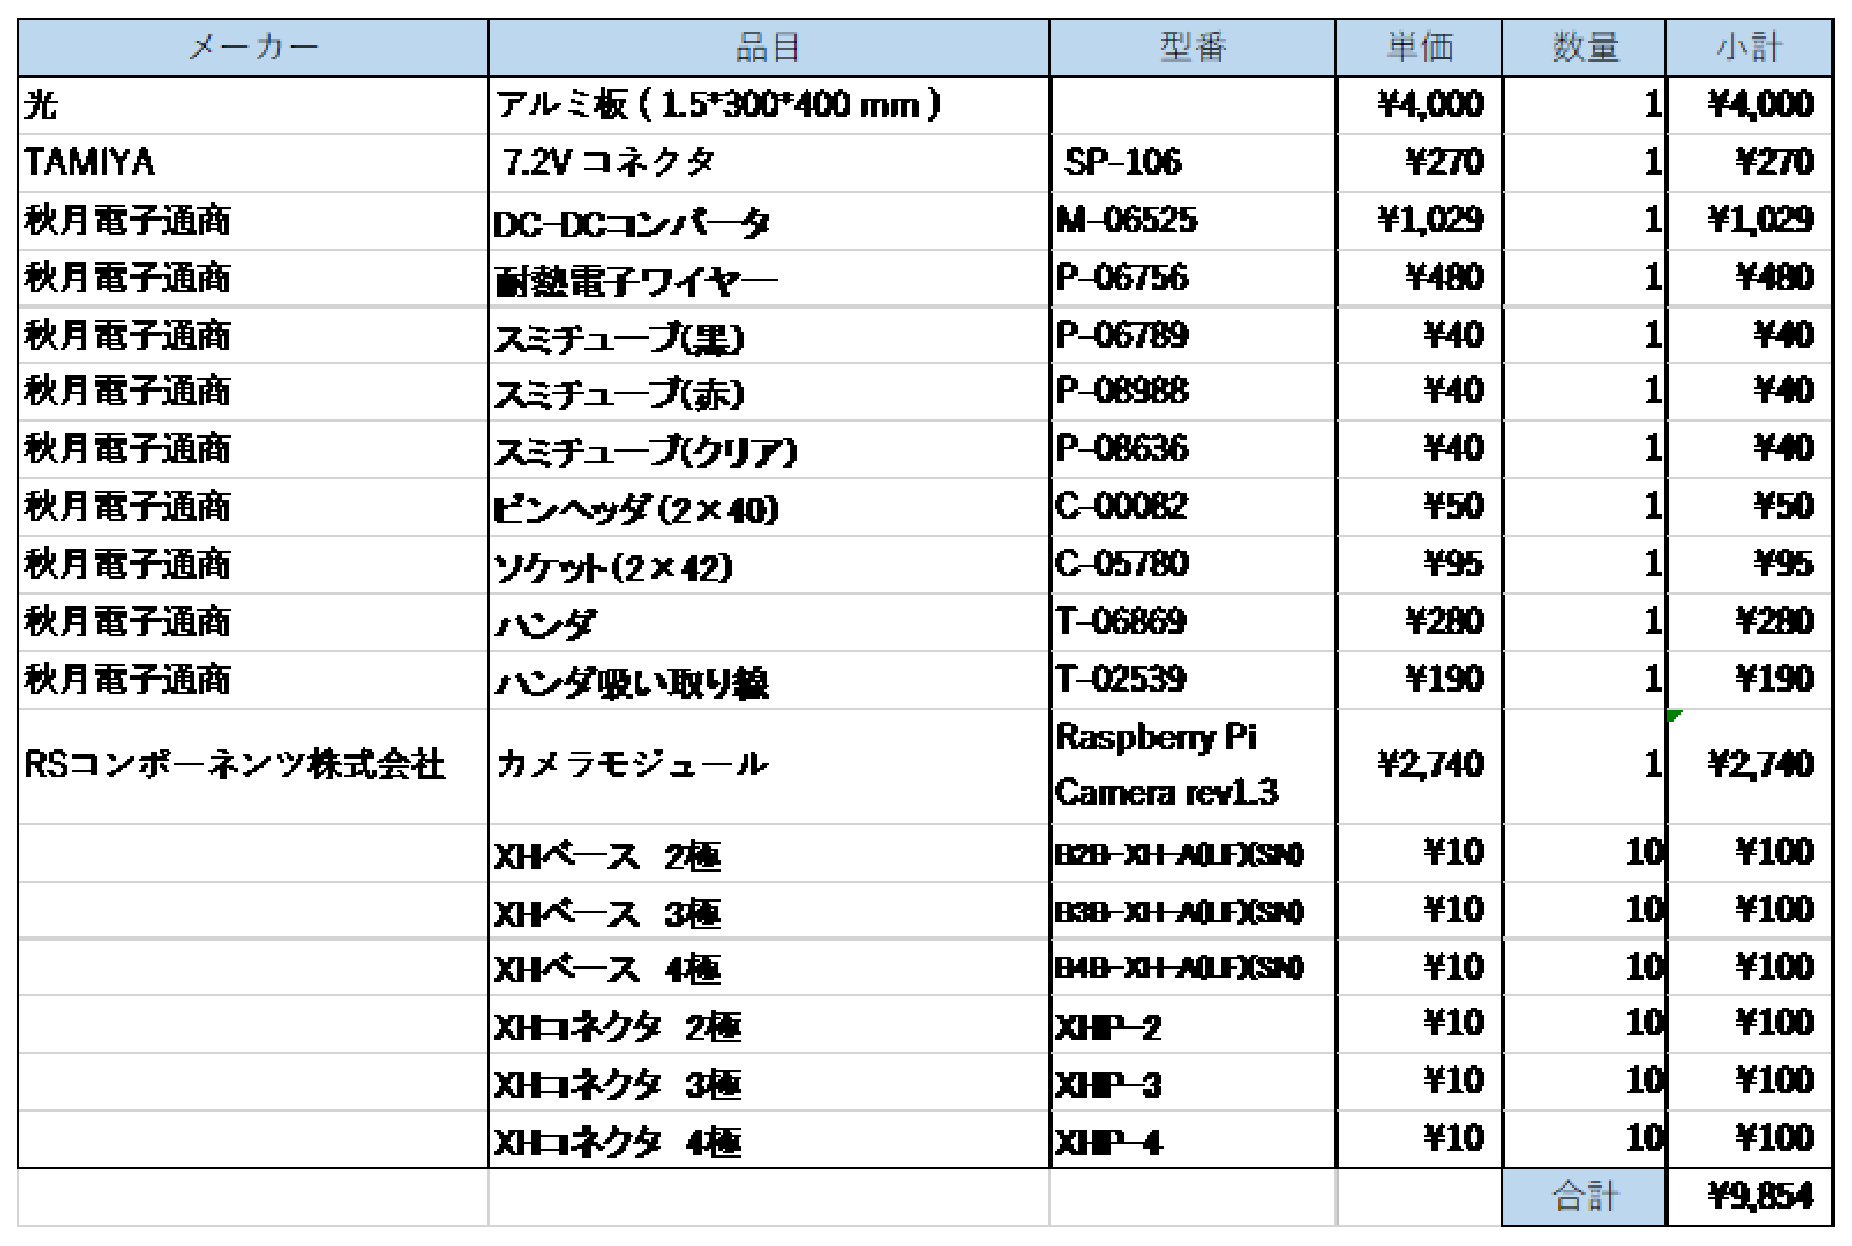
\includegraphics[width=1.0\hsize]{picture/items_distributed.eps}
  \end{table}

  \begin{table}[H]
    \centering
    \caption{購入品一覧}
    \includegraphics[width=1.0\hsize]{picture/items_purchased.eps}
  \end{table}

\newpage
\begin{thebibliography}{9}
  \bibitem{raspicam}
    "RaspiCam: C++ API for using Raspberry camera with/without OpenCV",\\
    "\texttt{https://www.uco.es/investiga/grupos/ava/node/40}",\\
    2017年5月31日最終確認.

  \bibitem{elinux}
    "RPi Camera Module - eLinux.org",\\
    "\texttt{http://elinux.org/Rpi\_Camera\_Module\#Technical\_Parameters\_.28v.2\_board.29}",\\
    2017年5月31日最終確認.
\end{thebibliography}

\end{document}

